\section{The Wolf-Goat-Cabbage Problem}

  \subsection{Question 1}

    Below is a graph representing the relationships between all possible states
    in the Wolf-Goat-Cabbage Problem. In this graphic:

    \bigskip
    \bigskip
    \noindent\makebox[\textwidth]{%

    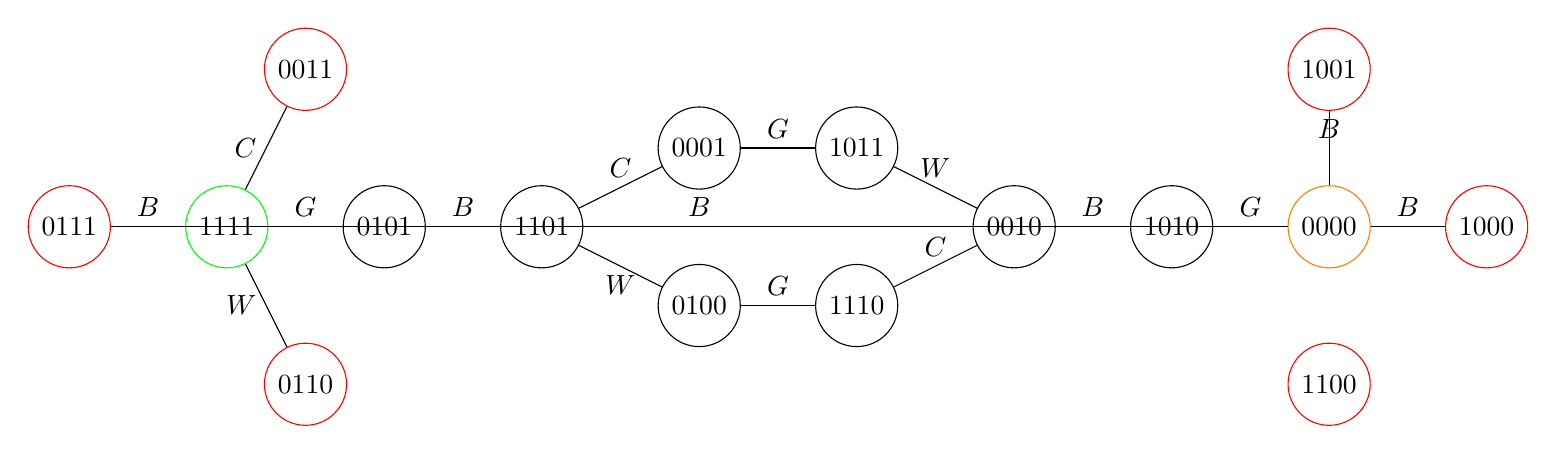
\begin{tikzpicture}[block/.style={circle}]

    \node[shape=circle, draw=orange] (0000) at (9,0) {0000};
    \node[shape=circle, draw=black] (0001) at (1,1) {0001};
    \node[shape=circle, draw=black] (0010) at (5,0) {0010};
    \node[shape=circle, draw=red] (0011) at (-4,2) {0011};
    \node[shape=circle, draw=black] (0100) at (1,-1) {0100};
    \node[shape=circle, draw=red] (0110) at (-4,-2) {0110};
    \node[shape=circle, draw=red] (0111) at (-7, 0) {0111};
    \node[shape=circle, draw=red] (1000) at (11,0) {1000};
    \node[shape=circle, draw=red] (1001) at (9,2) {1001};
    \node[shape=circle, draw=black] (1010) at (7,0) {1010};
    \node[shape=circle, draw=black] (1011) at (3,1) {1011};
    \node[shape=circle, draw=red] (1100) at (9,-2) {1100};
    \node[shape=circle, draw=black] (1110) at (3,-1) {1110};
    \node[shape=circle, draw=green] (1111) at (-5,0) {1111};
    \node[shape=circle, draw=black] (0101) at (-3,0) {0101};
    \node[shape=circle, draw=black] (1101) at (-1,0) {1101};

    \path [-] (1111) edge node[above] {$G$} (0101);
    \path [-] (1111) edge node[above] {$B$} (0111);
    \path [-] (1111) edge node[left] {$C$} (0011);
    \path [-] (1111) edge node[left] {$W$} (0110);

    \path [-] (0101) edge node[above] {$B$} (1101);

    \path [-] (1101) edge node[above] {$C$} (0001);
    \path [-] (1101) edge node[below] {$W$} (0100);

    \path [-] (0001) edge node[above] {$G$} (1011);
    \path [-] (0100) edge node[above] {$G$} (1110);

    \path [-] (1011) edge node[above] {$W$} (0010);
    \path [-] (1110) edge node[above] {$C$} (0010);

    \path [-] (0010) edge node[above] {$B$} (1010);

    \path [-] (1010) edge node[above] {$G$} (0000);

    \path [-] (0000) edge node[above] {$B$} (1000);
    \path [-] (0000) edge node[above] {$B$} (1001);
    \path [-] (0000) edge node[above] {$B$} (0111);

    \end{tikzpicture}
}


  \subsection{Question 2}

  Below is a tree representation of actions that may be taken to convert all
  actors being on one bank to another. Further, the error states (ie. all leaves that
  are not the goal state), are written $A \rightarrow B$, which reads as ``A
  consumes B''.

    \bigskip

    \noindent\makebox[\textwidth]{%
\Tree [.1111
  [.0111
    \textit{$G \rightarrow C$/$W \rightarrow G$}
  ]
  [.0011
    \textit{$W \rightarrow G$}
  ]
  [.0101 [.1101
    [.0001
      [.1001
        \textit{$W \rightarrow G$}
      ]
      [.1011
      [.0011
        \textit{$G \rightarrow C$}
      ]
      [.0010
        [. 1010 [. \textbf{0000} ]]
        [. 1110
            [. 0100
              [. 1100
                \textit{$G \rightarrow C$}
              ]
            ]
        ]
        ]
      ]
    ]
    [.0100
      [.1100
      	\textit{$W \rightarrow G$}
      ]
      [. 1110
        [.0110
          \textit{$G \rightarrow C$}
        ]
        [.0010
          [.1010
            \textbf{0000}
          ]
        ]
      ]
      [.1101
        [.0001
          [.1001
            \textit{$G \rightarrow C$}
          ]
        ]
      ]
    ]
  ]]
  [.0110
    \textit{$G \rightarrow C$}
  ]
]
}


  \subsection{Question 3}

    \bigskip

    $$1111 \rightarrow 0101 \rightarrow 1101 \rightarrow 0001 \rightarrow 1011
    \rightarrow 0010 \rightarrow 1010 \rightarrow 0000$$
